\documentclass{ou-report-vaf}

% Dit template is gemaakt door P.J. Molijn in het kader van zijn afstuderen aan de OU in 2014.
% Waarvoor hartelijk dank.
% Minieme maar belangrijke wijzigingen zijn aangebracht door E.M. van Doorn
% Het template is versimpeld door Sylvia Stuurman, 2019.
% Het template is aangepast voor de ba informatica door Harrie Passier, Tanja Vos en Pekka Aho 2020 

\def\mytitle{How can automated comparison of inferred models help testers finding bugs?}
\def\myauthor{Rick Neeft}

\begin{document}

    \pagenumbering{roman} 
%to prevent that the title page will be referred as page 1, 
%which will give the warning that there is a page 1 twice.

\pagestyle{plain}
\begin{titlepage}
    \begin{center}
    
        %% Insert the OU logo at the bottom of the page.
        \begin{tikzpicture}[remember picture,overlay]
            \node at (current page.south)[anchor=south,inner sep=0pt]{
                
\includegraphics[scale=0.7]{pics/OUlogo}
            };
        \end{tikzpicture}
        
        %% Extra white space at the top.
        \vspace*{2\bigskipamount}
        
        {\color{red}\Huge\bf \thetitle}
        \bigskip
        
        {\large Research proposal}
        
        \bigskip \bigskip
        by
        \bigskip \bigskip
        
        {\Large\bf \theauthor}
        
        \bigskip \bigskip\bigskip \bigskip
        
        \begin{tabular}{lll}
            %% Add additional information here, per faculty requirements, e.g
            Student number: & 851829973 \\
            Course code: & \textsc{IM}0502\\
            Thesis committee:
                & Prof. Dr. Tanja E.J. Vos (chairman), & Open University \\
                & Dr. Pekka Aho (supervisor), & Open University \\
                & Fernando Pastor Ricós (supervisor), & Universitat \\
                &  & Politècnica de València
        \end{tabular}
    
    \end{center}
\end{titlepage}
\pagenumbering{arabic} 

%to prevent that the title page will be referred as page 1, 
%which will give the warning that there is a page 1 twice.

\let\cleardoublepage\clearpage
    
    %This will automatically generate your table of contents
    \tableofcontents
    \newpage
    
    % Acronyms
    \printnoidxglossary[type=\acronymtype]
    \newpage
    
    \section{Introduction}
% I don't think I am making a correct point here.
"\textit{Software is everywhere and it’s filled with bugs}".\cite{filledWithBugs}\footnote{Says Marieke Huisman at her inaugural lecture\cite{filledWithBugs}}. The phones in our pockets, pacemakers in our body and guidance systems in space all run on software that is created by people. Most of the time it run without issues but if the software fails, it costs the society a lot of money. A report from Consortium for Information \& Software Quality (CISQ) \cite{herb2020cost} calculated that the cost for poor software quality in 2020 was \$2,08 trillion in the USA alone. When comparing the cost with a country's gross national income (GNI), it is the equivalent to the GNI of Brazil in 2019 \cite{worldbank}\footnote{Brazil had a GNI of \$1,92 trillion in 2019 \cite{worldbank}}. Not only the cost for poor software quality is high also the cost for verification and validation. 

%In addition to the cost of poor software quality, 20\% to 50\% of the cost of a development project is spent on verification and validation \cite{alegroth2016}. 

Due to the new development practices, like \acrfull{ci}, dev processes has speed up -> and time for testing decreased cite here. -> automation is therefore important and necessary. Continues integration (CI) speeds up the dev process which makes less that for testing

This document is structured as follows. Section \ref{background} describes the background of this proposal and contains information that is available but might not be known by students and readers. Section \ref{releatedWork} contains an overview of the material that can be seen as a direct foundation for this proposal. Section \ref{questions} formulates the research questions for the thesis, what is research method will be used and how the questions are being validated. The last section \ref{planning} will outline the planning for the GA-SE.
    \newpage
    
    \section{Background} \label{background}
This section describes the background of this proposal and contains information that is available but might not be known by students and readers. 

\subsection{Introduction into GUI Testing}
Ever since the first line of software is written, testers are testing its workings.While in the early day of software, the \acrfull{ui} was mainly terminals based or a set of blinking LEDs \cite{altair8800} \footnote{For example the ALTAIR 8800 computer \cite{altair8800}}, today we have an ever-increasing amount of \acrfull{gui} applications. Testings a GUI application is labour intensive and cost a lot of money. \cite{gui-history}

The first step in automation was to automate the work of the tester. This automation was accomplished by using Capture and replay (CR) software. A tester will record a test scenario into the CR software, and then the CR software will execute the test case when needed. Using CR software, the time needed to retest software decrease; however, the big downside is that when software changes, so must the recording scripts \cite{gui-history}.

\acrfull{mbgt} is the second step in automation. With MBGT, the GUI elements and behaviour is abstract on a higher level. The created models are used to generate abstract test cases. Those abstract test cases need to be mapped or transformed to get concrete test cases that are executed on the SUT. The downside of MBGT is the effort required to create the models and the need to have formal modelling expertise. Formal modelling expertise is not needed with the latest step in test automation: model inference. 

The \emph{model inference}, also known as model extraction and GUI Ripping \cite{gui-ripping}, is the current state-of-the-art approach to automate GUI testing \cite{gui-history}. Inferred models are state graphs based on the GUI of the SUT. There are two ways to generate inferred models; the first is a static approach where the source code of the SUT is used to create a GUI model. The second is a dynamic approach where the GUI state is captured and extracted while being executed. 

The static approach has several downsides. First, the source code must be available, which is not always the case and secondly, it is challenging to capture behaviour based on the GUI source code. For example, with HTML, it is easy to generate a model; however, its behaviour is either in Javascript or server code. Overcoming those downsides can be achieved by executing the SUT. 

The dynamic approach captures the model during test execution. The automated test tool interacts with the SUT in a scriptless of randomly exercising way. This random scriptless approach is called \emph{Monkey testing}. Usually, test monkeys have no idea in which state the SUT is in and what type of input is allowed. It is therefore essential to make the test monkey smarter. A 'smart test monkey' can be achieved by making "see" the UI elements (Section \ref{data-retrieval}). Section \ref{testar-testauto} will give more details about how TESTAR is using smart test monkeys.

\subsection{What is TESTAR?} \label{what-is-testar}
TESTAR - or TEST* - is an automated software testing tool for the GUI level \cite{testar-about}. TESTAR started within the context of the \acrfull{fittest} project. TESTAR is open-source, the source code is published on GitHub \footnote{ \url{https://github.com/TESTARtool/TESTAR\_dev}}. A screenshot of the TESTAR tool is displayed in figure \ref{fig:testar}.

\begingroup
\captionsetup{type=figure}
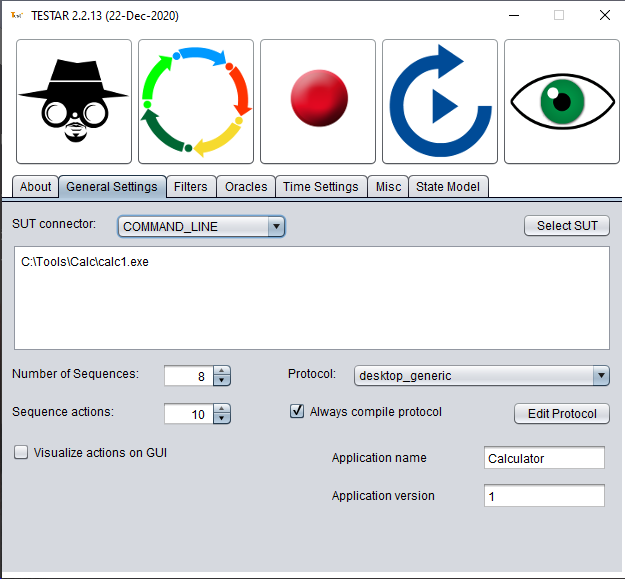
\includegraphics[scale=0.5]{pics/testar.png}
\captionof{figure}{Screenshot of the TESTAR tool}\label{fig:testar}
\endgroup

TESTAR has several \emph{execution modes} in which it interacts with the SUT \cite{testar-manual}. From left to right, in figure \ref{fig:testar}, those are Spy, Generate, Record, Replay and View mode. 

The \emph{Spy} mode allows the user to inspect a SUT and "see" how TESTAR is interpreting the widgets on the screen. Figure \ref{fig:calc-spy} shows the Windows calculator in spy mode. Dots on the GUI indicates actions with which TESTAR can interact. Within TESTAR, it is possible to filter actions. TESTAR will then not execute these actions. The actions are given a silver dot colour. A list with properties about the widget is shown when hovering, as well as a unique identifier of the current \emph{state}, more information about the state and the unique identifier can be found at section \ref{gui-state}.\par

\begingroup
\captionsetup{type=figure}
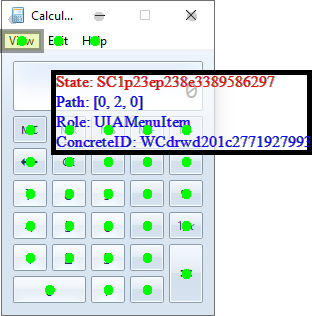
\includegraphics{pics/calc-state.png}
\captionof{figure}{Screenshot of the Calculator with TESTAR Spy}\label{fig:calc-spy}
\endgroup

In the \emph{Generate} mode will TESTAR will start testing the specified system. Section \ref{testar-testauto} for more detail about TESTAR test automation.

The \emph{Record} mode allows a tester to record a test sequence manually. In the \emph{Replay} mode, existing test execution can be re-executed and lastly, in the \emph{Review} mode allows existing test executions to be viewed.

\subsubsection{TEST automation} \label{testar-testauto}
TESTAR works without any test scripts but is uses GUI Ripper and Monkey testing techniques. \emph{GUI Ripping}, first introduced by Memon et al. \cite{gui-ripping} and is a process to obtain the GUI's structure and execution behaviour automatically. \emph{Monkey testing} is a process in which decisions (interactions with the GUI) are randomly chosen. Section \ref{data-retrieval} will give more insights into GUI Ripping.
TESTAR is using a flow to execute tests on the SUT. This flow is as follows:
\begin{enumerate}
    \item Start the SUT
    \item Scan the GUI and obtain the state (Section \ref{gui-state})
    \item Finding and selecting an action to execute
    \item Evaluate state with a test oracle (Section \ref{test-oracles})
    \item Stop the SUT when no actions are left to be executed or restart the SUT when more sequences are required.
\end{enumerate}

\begingroup
\captionsetup{type=figure}
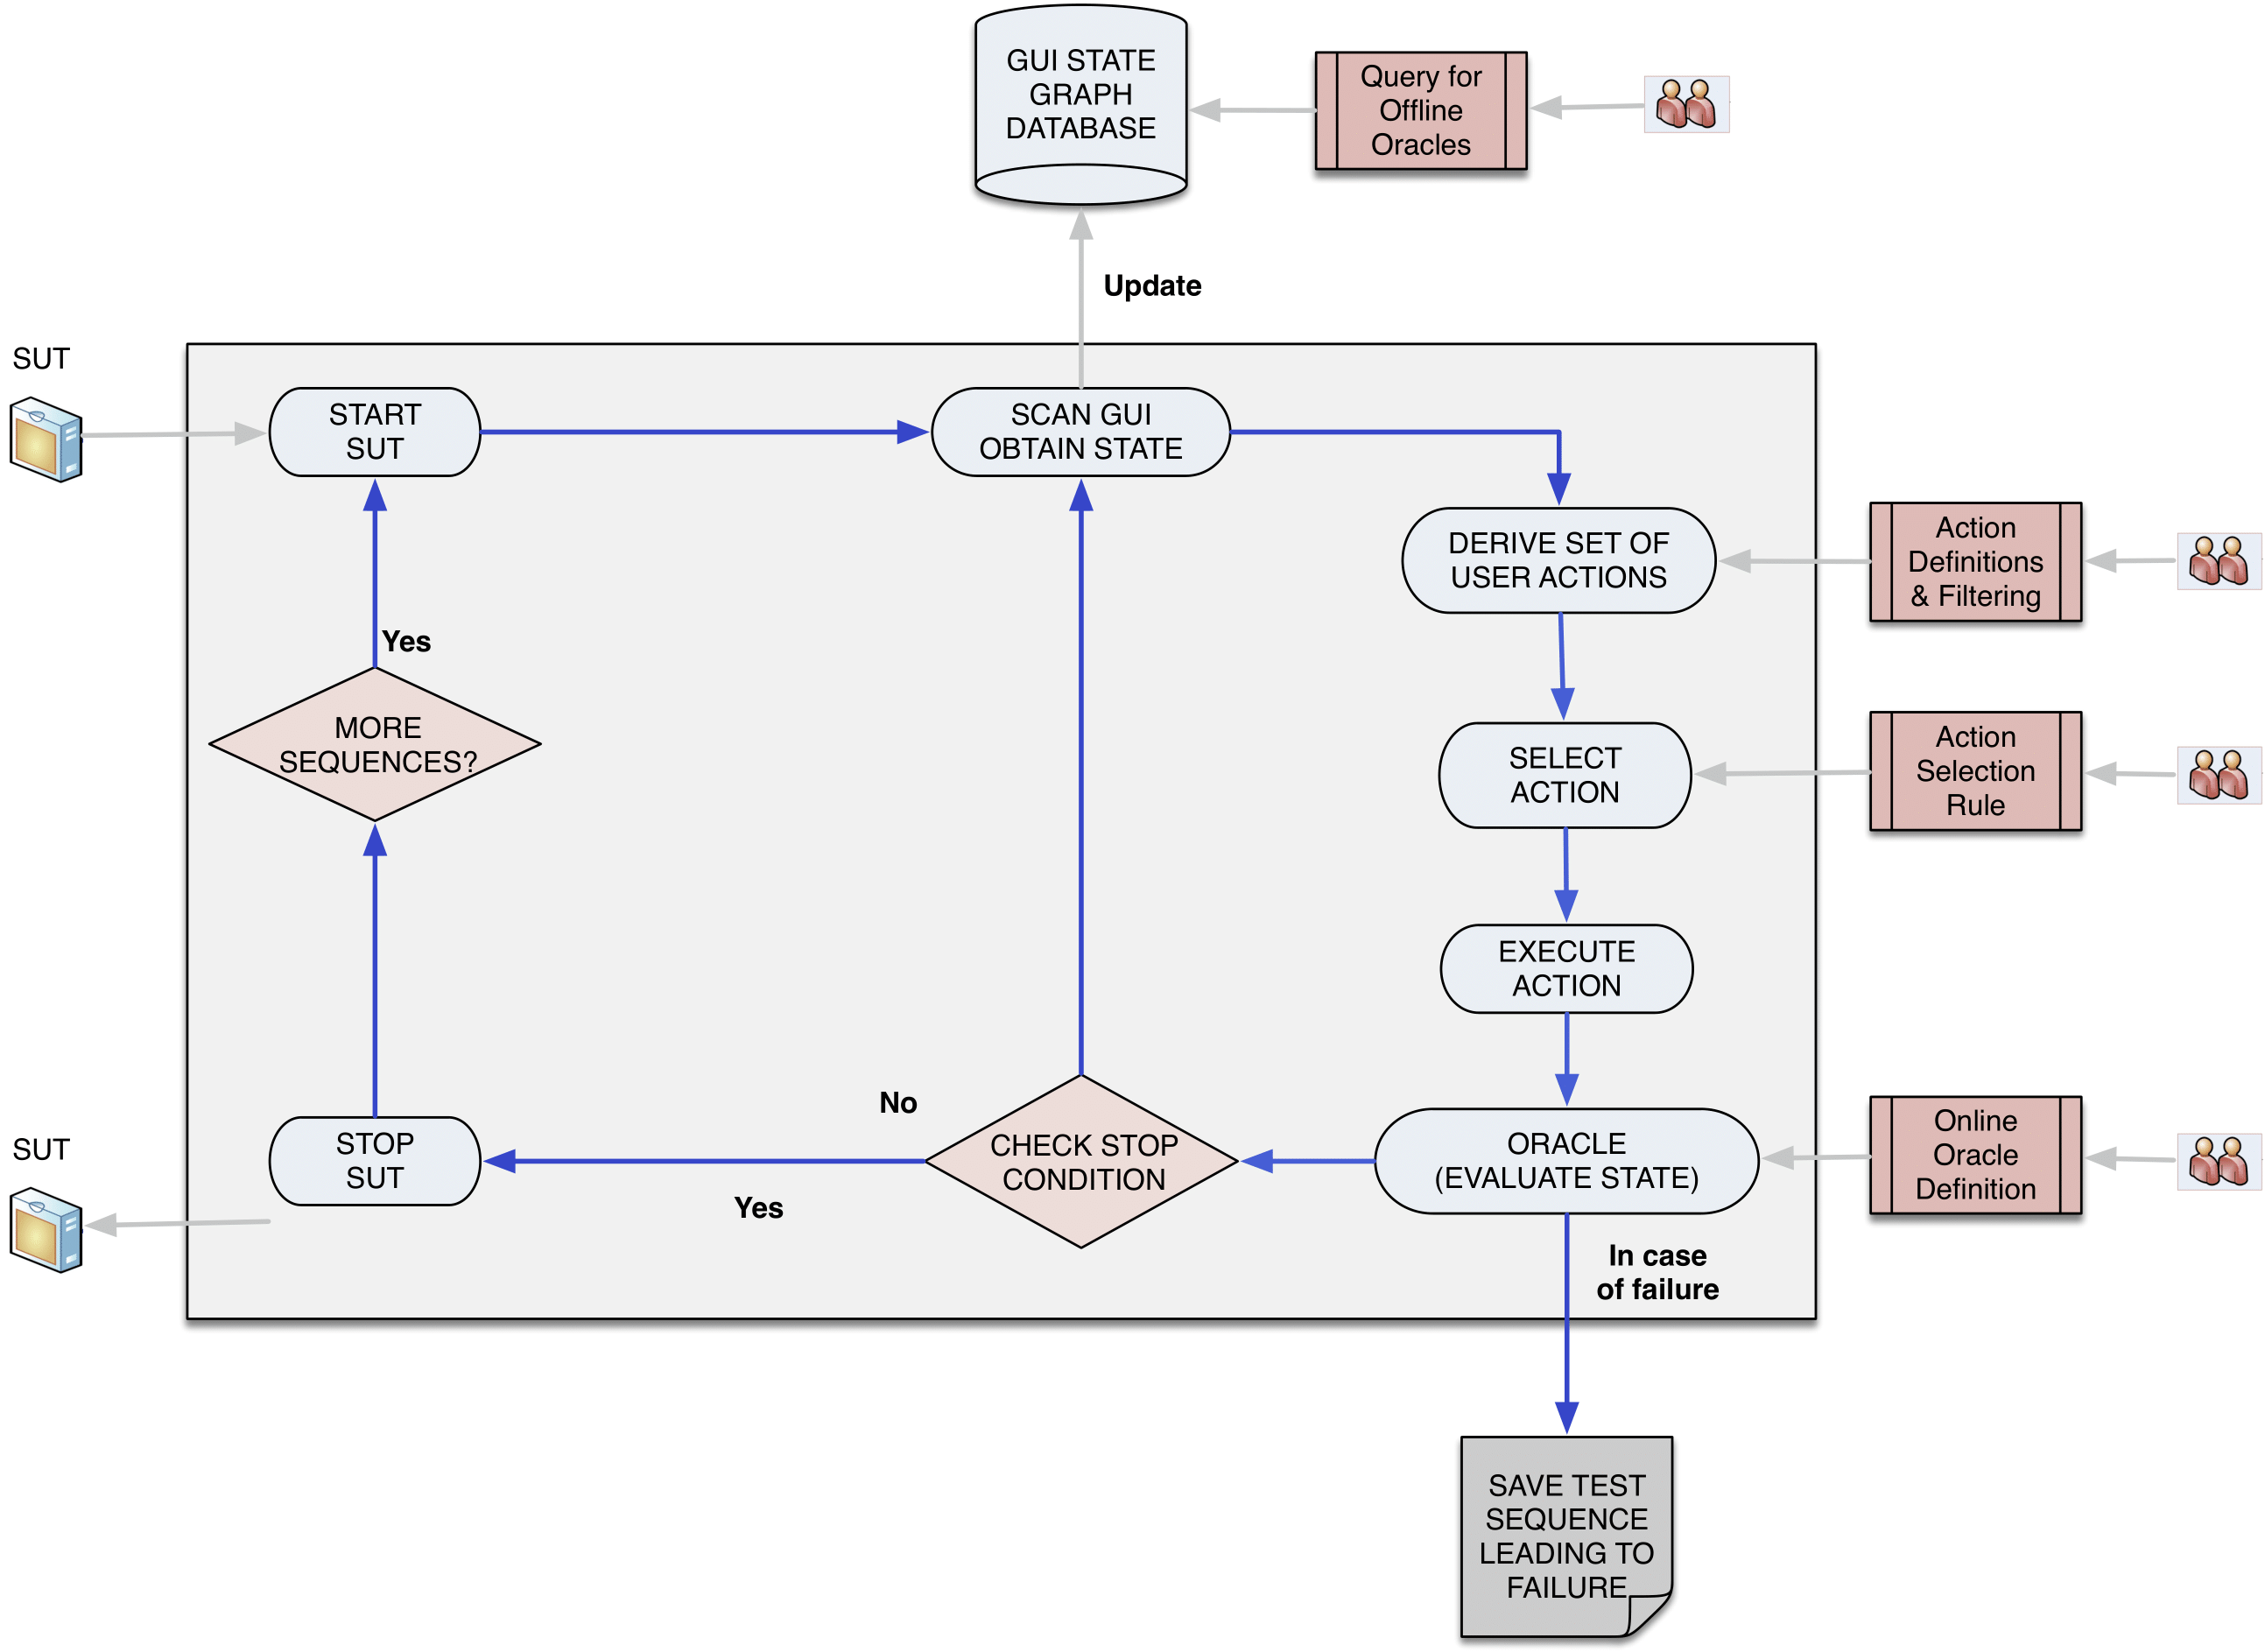
\includegraphics[scale=0.8]{pics/testar-test-cycle.png}
\captionof{figure}{TESTAR test cycle \cite{VosAho2021}}\label{fig:testar-test-cycle}
\endgroup

Figure \ref{fig:testar-test-cycle} show the flow graphically \cite{VosAho2021}. TESTAR manages everything inside the grey box. The test specialist needs to provide SUT details to TESTAR like which actions should not be executed, select a selection mechanism, and they should define which SUT behaviour is correct and which is not (Section \ref{test-oracles}). 

\subsection{How is the SUT tested} \label{test-oracles}
When software is tested, a method is needed to check the correct behaviour of the SUT. The method of checking is formally known as a \emph{test oracle} \cite{testOracles}. An example of a test oracle widely used by developers is the code \emph{assertions}, which is a Boolean assertion. Developers can create assertions in software to check its behaviour during runtime \cite{barr2014oracle}. Assertions can also be used in unit tests as displayed by listing \ref{code:assert}. 

%% do not indent code since it indents its extra in the LaTeX output
\begin{lstlisting}[language=Java, caption=Assertion, label=code:assert]
@Test
public void testAdd(){
    Calculator sut = new Calculator();

    int expected = 3;
    int actual = sut.Add(1,2);

    Assert.assertEquals(expected, actual);
}
\end{lstlisting}

\subsubsection{Online and Offline Test oracles}
Test oracle comes in two variants, \emph{online} or \emph{on-the-fly} test oracle and \emph{offline} test oracles \cite{VosAho2021}. With online test oracles, the state under test is being asserted for any anomalies during test execution. For example,  an online test oracle inspects the URL to check for any information being exposed in the query string. Offline test oracles will look into stored data - like logs - to find anomalies after test execution. For example, offline test oracles can inspect all the visited URL's to check for any exposed information in the query strings.

Each variant come with their strengths and weaknesses. The online test oracle takes up compute time because it inspects the state during test execution. This inspecting of state slows down the test execution and may become an issue with time-critical SUT's. On the other hand, some issues - like the SUT become unresponsive - can only be checked during test execution. An offline test oracle is inspecting data that is gathered when test execution has finished. Especially with larger data sets, this can become helpful. Inspecting the data may run in parallel, which can speed up the test oracle. Additionally, when developers create new offline test oracles, they can inspect the recorded data instead of executing a new test run. \cite{de2019offline}

\subsection{How is data retrieved} \label{data-retrieval}

Section \ref{testar-testauto} discussed how TESTAR is using GUI ripping to obtain the GUI's structure. A GUI exists out of a non-empty set of UI components, known as \emph{widgets}. Examples of widgets is a Window or a button; more examples can be found in table \ref{tables:widgets} \cite{VosAho2021}. The widgets are structured hierarchy in a \emph{widget tree}. Each node in the tree is a widget with its related properties, such as the title, position, and role.

\begingroup
\captionsetup{type=table}
\begin{tabularx}{\textwidth}{ 
  | >{\raggedright\arraybackslash}X 
  | >{\raggedright\arraybackslash}X 
  | >{\raggedright\arraybackslash}X | }
    \hline
    Windows & Menus & Controls \\
    \hline
    \hline
    main windows & menu bars & buttons \\
    child windows & dropdown menus & textbox \\
    popup windows & context-aware menus & links \\
    && radio buttons \\
    && checkboxes\\
    && dropdown select boxes\\
    && sliders\\
    && tabs\\
    && scrollbars \\
    \hline
\end{tabularx}
\captionof{table}{Example of GUI widgets \cite{VosAho2021}}\label{tables:widgets}
\endgroup

 The widgets are structured hierarchy in a \emph{widget tree}. Each node is a widget with its corresponding properties inside the tree, such as the title, position, and role. In figure \ref{fig:widget-tree} a compact widget tree is shown for the calculator. 

\begingroup
\captionsetup{type=figure}
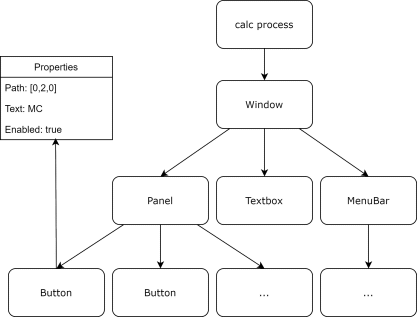
\includegraphics{pics/calc-tree.png}
\captionof{figure}{A compact version of a widget tree for the calculator.}\label{fig:widget-tree}
\endgroup

\subsection{Widget data API}

In order to retrieve data from a SUT, TESTAR is making use of external API's to access widgets that are part of the GUI \cite{thesisMulders}. TESTAR is using three different API's.

In order to test desktop application, TESTAR makes use of the Windows Automation API. The purpose of the Windows Automation API is to expose rich information about UI elements\cite{win-api-info}. For web applications, TESTAR uses Selenium Chromedriver. The Chromedriver is a tool for automated testing. It provides capabilities for navigating web pages, user input, and JavaScript execution \cite{chrome-driver-info}. The latest API that TESTAR is using is Appinum. Appinum is a test automation tool for native, mobile web, and hybrid applications on iOS mobile, Android mobile, and Windows desktop platforms \cite{apinum-info}

\subsubsection{GUI State} \label{gui-state}

The title of this research proposal is \emph{"\mytitle"}. An inferred model is a directed graph with state and actions. Each vertex represents the application's state, a snapshot of the visible GUI when no actions are executed, \cite{gui-history, thesisMulders} and the edges represent an action, like pressing a button. Figure \ref{fig:state-example} shows an example of a graph created for the Windows calculated (UI elements have been trimmed for space purposes).

\begingroup
\captionsetup{type=figure}
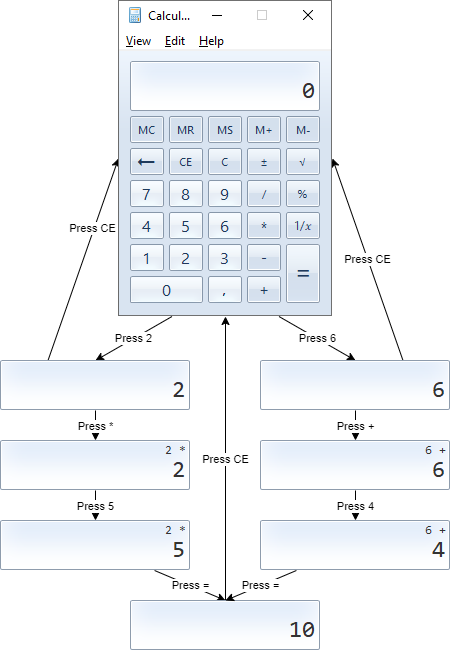
\includegraphics[scale=0.5]{pics/calc-state-example.png}
\captionof{figure}{An example state graph for the Windows Calculator.}\label{fig:state-example}
\endgroup

A directed graph with each vertex a screenshot of the SUT is an example of the \emph{Murphy} tool's output. \emph{Murphy} is developed by a software company from Finland (F-Secure) that can be used to extract GUI models for testing GUI applications automatically. \cite{aho2013industrial}. Although the context for the research is TESTAR, Murphy can be research to learn how it detects changes and apply that knowledge to TESTAR \cite{murphy-extract-gui}.

To identify the state (and actions), TESTAR calculates two state identifiers; an abstract and concrete state identifier \cite{thesisMulders}. For the concrete state identifier, all the properties of a widget are used. For the abstract identifier, a subset of the properties is used. It is configurable which properties are used for the abstract identifier. By default the properties \textit{role}, \textit{title}, \textit{position} and \textit{enabled} are used.

TESTAR uses the following hashing algorithm: For each widget, the used properties are concatenated and hashed. Those hashed are then joined and hashed to retrieve the hash used to identify the state.

\subsection{How is data persisted}

TESTAR is using a database to store and retrieve state model data. Gier and Kager investigated which data storing solution would be beneficial to TESTAR \cite{GierKager}. The data solution must comply with six requirements. Generally speaking, the requirements were as follows: an open-source graph database with a straightforward query mechanic. The conclusion was that OrientDB was the best solution that met all the requirements.

OrientDB is a Multi-Model NoSQL \acrfull{dbms} that combines four models \cite{orientDbModeling}:

\begin{itemize}
    \item \hyperlink{db:key-value}{Key/Value}
    \item \hyperlink{db:document}{Document}
    \item \hyperlink{db:graph}{Graph}
    \item \hyperlink{db:object}{Object}
\end{itemize}

A \hypertarget{db:key-value}{\emph{Key/Value}} is the simplest model and allows storing information (value) that is accessible with a key. Key/Values can be group into \textit{buckets} however, OrientDB support richer models in the form of document and graph elements.

A \hypertarget{db:document}{\emph{document}} is a schema-less set of key/value pairs. The \emph{key} allows access to the corresponding value. OrientDB allows the developer to store documents into \emph{clusters}. Relations between document are either embedded into other document or \emph{linked} to each other. Someone familiar with relational databases can view a cluster as tables, a document as the row and the key/value pairs are columns.

The \hypertarget{db:graph}{\emph{graph}} is a model consisting of \emph{Vertices} and \emph{Edges}. Vertices are the nodes in the graph, and the edge is the link between those nodes. In TESTAR terminology, a vertex represents state, and the edge is an 'action' from one state to the next. A Vertex consists of three elements: a unique identifier, a set with incoming Edges and outgoing Edges. An edge consists of four elements: a unique identifier, an incoming vertex (\emph{head}), an outgoing vertex (\emph{tail}) and a label that describes the relationship between the head and tail vertex.\par

The last model is the \hypertarget{db:object}{\emph{object}}, which supports inheritance like in the Object-Oriented programming paradigm.\par

Despite being a NoSQL database, OrientDB does support SQL as a query language \cite{sql-lang} albeit that it does not support all SQL statements. The majority of developers have experience with SQL \cite{sql-stats} as a result, new developers and students can start querying the TESTAR data and start expanding its features.\par

In addition to TESTAR, other applications can query the state model data in the OrientDB database as well. For example, developers and students can create external tools for a single purpose, like a state model difference application. When building external tools, the TESTAR application can be kept small and focus upon one objective: testing GUI applications. 
    \newpage
    
    \section{Related work} \label{releatedWork}
    
    This section covers an overview of the material that can be seen as the direct foundation for this proposal.
    
    \subsection{Inferring state models in TESTAR}
    
        In a recent student master graduation project, Inferring state models in TESTAR, \cite{thesisMulders}  the foundation is created to build state models with TESTAR. The result can be found inside the \verb|StateModel| package\footnote{\url{https://github.com/TESTARtool/TESTAR_dev/tree/master/testar/src/nl/ou/testar/StateModel}}
        -> is saved in an OrientDB database - > which gives good query options -> viewer is build to see the model. 
        
        Future work might be adding unit test on the part that will be touched since no code coverage has been found for the package.

        %What is a state 3.3
        
        %\subsubsection{State of the source code}
        
        %Mulders concluded in his thesis \cite{thesisMulders} that 
        


    \subsection{State model difference}
        The \verb|StateModel.Difference| package was added by Ricós\cite{stateDiff} and offers a proof of concept for calculating differences between the state models of two versions. 
        
        Ricós started with a proof of concept for state model difference \footnote{\url{https://github.com/TESTARtool/TESTAR_dev/tree/state_model_difference}}
        give two sut version -> calculates difference in added and removed states.
        
        Let $A$ be a set of states of version 1 of the SUT, let $B$ be a set of states of version 2 of the SUT. The removed states can be written as
        \[A-B = \lbrace x | x \in A \wedge x \notin B \rbrace\]
        the states that are added can be written as
        \[B-A = \lbrace x | x \in B \wedge x \notin A \rbrace\]
        
        Future work can be viewing the SUT en all version as a universe of states to see which states are removed and added, maybe moved (if location is not part of the state)
        
        Future work -> adding unit tests since those are not present -> refactoring of the code since some file do not have a clear Separation of concern. -> one can observation the return and input values are form of \verb|string| (e.g. \verb|string| \verb|Set<String>| etc) -> can lead to primitive obsession -> investigation is needed to solve this. 

    \newpage
    
    \section{Research} \label{questions}
    In this section the research questions for the thesis are formulated. What is research method will be used and how the questions are being validated.

    \subsection{Context}
    What is the context of the research. 
    
   % Creation of test oracles are out of scope.
    
    % due to the experiment below sentence is false
    %The main research question will be around finding bugs with two inferred models. Even though generating models is needed, no research will be executed on generating those.
    
\subsection{Research questions}
        
The main research question is: \textbf{How can an automated comparison of inferred models help testers finding bugs?}

The main research questions divided into two parts. The first part (\ref{rq:detect-changes}) will research how to detect changes between versions of the same GUI software (SUT)?\cite{testar-todo}. The second part (\ref{rq:diff-visualisation}) will research how to visualise the detected changes. The research questions are as follows: 

\begin{questions}
    \item How to detect changes between two versions of the SUT? \label{rq:detect-changes}
    \begin{questions}
        \item What requirements are there for the inferred model for change detection? \label{rq:model-requirements}
        \item What is a useful model for change detection? \label{rq:useful-model}
        \item Which configuration will generate a useful model? \label{rq:gen-useful-model}
        \item Which classification can be given to a difference in a state model? \label{rq:classifications} 
        \item Which algorithm can be used to detect differences between state diagrams? \label{rq:difference-algorithm}
    \end{questions}

    \item How to visualise the detected differences to the user? \label{rq:diff-visualisation}
    \begin{questions}
        \item What tooling is available to show the detected differences? \label{rq:tooling}
        \item How to visualise each type of change? \label{rq:type-visualisation}
        \item How to generate the shortest set with actions that helps the user to reach the changed state in the SUT? \label{rq:shortest-set}    
    \end{questions}

\end{questions}

\subsubsection{\ref{rq:model-requirements} What requirements are there for the inferred model for change detection?}
The outcome of \ref{rq:model-requirements} is a list of requirements for the inferred model that are needed to enable change detection. For example, can a non-deterministic state model be used? However, it also includes requirements for the algorithm, like, what are acceptable calculation speeds and how big can a state model be while still complying with the speed requirement. 

\subsubsection{\ref{rq:useful-model}What is a useful model for change detection?}
In the master thesis, Mulders asked the question "\textit{What makes a model useful for TESTAR's purpose}" \cite{thesisMulders}. He used the Vaandrager's criteria \cite{vaandrager} to answer that question. To validate the requirements from RQ \ref{rq:model-requirements} the Vaandrager's criteria will be used. 

\subsubsection{\ref{rq:gen-useful-model} Which configuration will generate a useful model?}
There are a couple of ways to change the outcome of an inferred model, for example, picking widget attributes for the hash calculation. These configurations can influence the usefulness of the model. The outcome of \ref{rq:gen-useful-model} should result in a TESTAR configuration file that configures TESTAR to generate this useful model. It might be necessary to make code changes in the state model generation.

A thread of validity for \ref{rq:gen-useful-model} is that every application under test needs its unique configuration. Therefore it might be wise to look into all widgets attributes during the change detection and not take the hash of a state for the comparison. The configuration can be used for tuning the model and the change detection by taking the above approach.

\subsubsection{\ref{rq:classifications} Which classification can be given to a difference in a state model?}
The current algorithm \cite{stateDiff} makes two classifications regarding differences in state diagrams; added and removed state. As a consequence, two state changes are observed when an action in the \acrshort{sut} is moved. For instance, an about window is moved from the \verb|File| to the \verb|Help| menu. The hypothesis of \ref{rq:classifications} is that it can help the tester understand what kind of change is made to a new version of the \acrshort{sut}.

\subsubsection{\ref{rq:difference-algorithm} Which algorithm can be used to detect differences between state diagrams?}
\ref{rq:difference-algorithm} is the closing question in which the algorithm is coded in Java. In a recent master thesis by Slomp \cite{insert-slomp-hereTODO}, it is possible to run TESTAR in a Docker container. As a consequence, TESTAR can run without a GUI. Therefore the change detection algorithm will run in a separate application, outside the TESTAR context. The result of the change detection needs to be saved to the already existing OrientDb database. 

\subsubsection{\ref{rq:tooling} What tooling is available to show the detected differences?}
Aside from the inferred model, Mulders also created an application to visualise the models. It is essential to state that Mulders did extensive research on which technology fits his needs best. \ref{rq:tooling} will look at the results of Mulders and revalidate whether the libraries are useable to visualise differences. 

\subsubsection{\ref{rq:type-visualisation} How to visualise each type of change?}
\ref{rq:type-visualisation} will look into the execution of the visualisation tool. Like \ref{rq:difference-algorithm} this also include moving the visualisation tool into its own application, outside the TESTAR context. The requirements and GUI proposals will be discussed with the TESTAR stakeholders. 

\subsubsection{\ref{rq:shortest-set} How to generate the shortest set with actions that helps the user to reach the changed state in the SUT?}
One of the requirements of the visualisation is showing how to reach the state is has changed. Dijkstra's algorithm \cite{dijkstra1959note} is a well-known algorithm to find the shortest path for a given graph. However, as Goldberg and Harrelson \cite{goldberg2005computing} showed, it is not the most optimal short path algorithm, especially with massive graphs. 


    \subsection{Research method}
    
       % A literature study will be conducted for \ref{rq:algorithm} and \ref{rq:differenceTool}. 
        
        % add starting papers for each research question.
        
    \subsection{Validation}
    
        %We can also test the outcome of TESTAR by infering models of the same version SUT and comparing those two models. Those two models should not contain any differences. 

        %A thread to conclusion of \ref{rq:differenceTool} can be that researches or companies are trying to sell a product -> therefor write material which favors their product -> With all material assessing the objectivity of the material is of great importance. -> Might need to express the favor of the current viewer \cite{thesisMulders} but that could downgrade the conclusion of \ref{rq:differenceTool}. 
    
    \newpage
    
    \section{Planning} \label{planning}

Planning is complex, and planning a graduation project with every detail included is near to impossible. To ensure the project is heading in the right direction, we will adopt an Agile, iterative approach that resembles the SCRUM methodology. Adopting the SCRUM methodology as a whole is, for a one-person team, overkill. However, some parts of the SCRUM methodology will be adapted. 

\subsection{Iterative approach} \label{iterative-approach}
\begin{displayquote}
Plans are worthless, but planning is everything
-Dwight D. Eisenhower \cite{agile}
\end{displayquote}

Although an iterative approach, called sprints in SCRUM, makes it possible to incorporate lessons learned into new decisions and tasks, having a plan or roadmap is still essential. In section \ref{deliverables}, the deliverables for the graduation project are defined. 

The graduation project consists of roughly 28 weeks (15 EC * 28 hours / 15 hours a week). Considering that one sprint is defined as two weeks, it is possible to conduct 14 sprints. 

\subsection{Control mechanism} 
Undoubtedly there will be moments where not everything goes according to plan. For this reason, a control mechanism is in place. The supervisors and the student will conduct a weekly meeting. At every start of a new iteration, the work for the sprint is planned. The iteration will end with a demo of the results and a retrospective, what went good and what can be done better. Considering that only one person will execute the project, the demo and planning sessions are held in one meeting, taking roughly 45 minutes to an hour. During an iteration, the committee will have a short meeting to assess the mid-iteration process and discuss any impediments. This meeting will take roughly 15 minutes. 

To summarise: the graduation project consists of 14 sprints. One sprint is two weeks. As the control, a weekly meeting is in place to discuss the progress and a demo and planning meeting at the end/start of the sprint. 

\pagebreak
\subsection{Deliverables} \label{deliverables} 
The deliverables are as follows:
\begin{itemize}[noitemsep]
    \item A Stand-alone application to execute the change detection,
    \item a stand-alone application that visualises the changes between two versions of the SUT,
    \item the Thesis,
    \item GA presentation.
\end{itemize}

\subsection{Roadmap} \label{roadmap}
The roadmap is defined in five work items: epics, features, product backlog items, bugs and tasks. A detailed explanation of these categories is giving in table \ref{tables:workitems-explanation}.

\begingroup
\captionsetup{type=table}
\begin{tabularx}{\linewidth}{ 
  | >{\raggedright\arraybackslash}l
  | >{\raggedright\arraybackslash}X  |}
    \hline
    Type & Explanation \\
    \hline
    \hline
    
    \emph{Epic} & An epic represents a goal of the graduation project. For each main research question (\ref{rq:detect-changes}, \ref{rq:diff-visualisation} and \ref{rq:validation}) an epic is created. An epic contains a non-empty set of features \cite{epics-features}.\\
    \hline

    \emph{Feature} & A feature represent a shippable component of the software or part of the thesis. A feature contains a non-empty set of product backlog items \cite{epics-features}. \\
    \hline
    
    \emph{Product Backlog Item} & A \acrfull{PBI} represents a requirement or element for the application. When a PBI is planned, the developer creates tasks \cite{user-story}. \\
    \hline
    
    \emph{Task} & A task is the smallest unit of work. Usually, the tasks are created ad-hoc and are used to keep track of the work of a PBI.  \\
    \hline

    \emph{Bug} & The work item Bug reflects a defect in the code and are handled the same as a PBI. When someone finds an issue with the code, it is registered as a bug and planned accordingly.\\
    \hline
\end{tabularx}
\captionof{table}{Five type of work items }\label{tables:workitems-explanation}
\endgroup

The planning in sprints can be viewed in table \ref{tables:sprints}, assuming the Graduation project starts on 29 August 2021, and weekly meetings are held on Thursdays. The sprint always ends on Wednesdays and start on Thursdays. There are more sprints planned than the (14) sprints estimated in section \ref{iterative-approach} to compensate for holidays in October-November and Christmas. 

\bigskip
\begingroup
\captionsetup{type=table}
\begin{tabularx}{\linewidth}{ 
  | >{\raggedright\arraybackslash}X |
  | >{\raggedright\arraybackslash}X |
  | >{\raggedright\arraybackslash}X  |}
    \hline
    Name & Start date & End date\\
    \hline
    \hline
  Sprint 01&26/Aug/2021&08/Sep/2021\\	 
 \hline
  Sprint 02&09/Sep/2021&22/Sep/2021\\	 
 \hline
  Sprint 03&23/Sep/2021&06/Oct/2021\\
 \hline
  Sprint 04&07/Oct/2021&20/Oct/2021\\	 
 \hline
  Sprint 05&21/Oct/2021&03/Nov/2021\\	 
 \hline
  Sprint 06&04/Nov/2021&17/Nov/2021\\	 
 \hline
  Sprint 07&18/Nov/2021&01/Dec/2021\\	 
 \hline
  Sprint 08&02/Dec/2021&15/Dec/2021\\	 
 \hline
  Sprint 09&16/Dec/2021&29/Dec/2021\\	 
 \hline
  Sprint 10&30/Dec/2021&12/Jan/2022\\	 
 \hline
  Sprint 11&13/Jan/2022&26/Jan/2022\\	 
 \hline
  Sprint 12&27/Jan/2022&09/Feb/2022\\	 
 \hline
  Sprint 14&10/Feb/2022&23/Feb/2022\\	 
 \hline
  Sprint 15&24/Feb/2022&09/Mar/2022\\	 
 \hline
  Sprint 16&10/Mar/2022&23/Mar/2022\\	 
 \hline
  Sprint 17&24/Mar/2022&06/Apr/2022\\	 
 \hline
  Sprint 18&07/Apr/2022&20/Apr/2022\\	 
 \hline
\end{tabularx}
\captionof{table}{Sprint planning}\label{tables:sprints}
\endgroup

\subsubsection{Epic \& Features}
Table \ref{tables:epics} and \ref{tables:features} are showing the epics and features for the project. Because an existing planning tool is used for the planning of this project, the IDs are not starting at 0.
\bigskip

\begingroup
\captionsetup{type=table}
\begin{tabularx}{\linewidth}{ 
  | >{\raggedright\arraybackslash}l |
  | >{\raggedright\arraybackslash}X |}
    \hline
    Id & Title\\
    \hline
    \hline
    356 & [RQ1] Detecting changes between two version of the SUT\\
    357 & [RQ2] Visualise changes to the user\\
    358 & [RQ3] Validate RQ1 and RQ2\\
    397 & Finish Graduation assignment\\
    \hline
\end{tabularx}
\captionof{table}{Epics}\label{tables:epics}
\endgroup

The list of epics can be found on: \href{https://dev.azure.com/chroomsoft/Study/_backlogs/backlog/Study Team/Epics}{Azure DevOps - Epics}
\bigskip

\begingroup
\captionsetup{type=table}
\begin{tabularx}{\linewidth}{ 
  | >{\raggedright\arraybackslash}l |
  | >{\raggedright\arraybackslash}X |
  | >{\raggedright\arraybackslash}l |}
    \hline
    Id & Title & Parent Id\\
    \hline
    \hline
    364 & Move code into the visualisation container  & 356\\
    387 & What is change detection & 356\\
    408 & Add change detection application as dependency to TESTAR & 356\\
    377 & Add database sign in to website & 357\\
    359 & Visualise tool should operate inside its container  & 357\\
    369 & Visualise each change & 357\\
    391 & Validate results in business environment & 358\\
    380 & Develop change detection algorithm & 356\\
    367 & What is a useful model & 356\\
    386 & Store change detection outcome in database & 356\\
    414 & Validate own tool & 358\\
    382 & Look for open-source application for validation & 358\\
    376 & Add REST API functionality & 357\\
    372 & Show user how to navigate to a change & 357\\
    398 & Finish Thesis & 397\\
    399 & GA presentation & 397\\
    \hline
\end{tabularx}
\captionof{table}{Features}\label{tables:features}
\endgroup
The list of features can be found on: \href{https://dev.azure.com/chroomsoft/Study/_backlogs/backlog/Study Team/Features/}{Azure DevOps - Features}

\newpage
\subsubsection{Product Backlog Items}
Table \ref{tables:product-backlog-items} shows all the PBIs for the project in order they are planned to be completed.
\bigskip

\begingroup
\captionsetup{type=table}
\begin{tabularx}{\linewidth}{ 
  | >{\raggedright\arraybackslash}l |
  | >{\raggedright\arraybackslash}X |
  | >{\raggedright\arraybackslash}l |}
    \hline
    Id & Title & ParentId\\
    \hline
    \hline
   365 & Move the POC code of Fernando to the visualisation container & 364\\
    366 & Add system (unit) test to the code base & 364\\
    406 & Add CI/CD pipeline to change detection application & 364\\
    381 & Study change detection & 387\\
    407 & What other forms of change detection are out there & 387\\
    409 & How to add dependency to TESTAR & 408\\
    378 & Make sure user can sign in to the site & 377\\
    410 & Add application model selection screen to application & 359\\
    375 & Implement "change report" into the visualisation tool & 369\\
    392 & Ask F-Secure for feedback & 391\\
    411 & How to detect changes between two version of a SUT & 380\\
    412 & Which properties need to be enabled for TESTAR to generate useful model & 367\\
    388 & Reflect model with Vaandrager criteria & 367\\
    393 & Implement change detection algorithm & 380\\
    396 & How to store the outcome of the change detection & 386\\
    413 & Saving change detection results & 386\\
    415 & Setup TESTAR for validation application & 414\\
    360 & Move visualise code to it own container & 359\\
    362 & Add system (unit) tests for visualisation code & 359\\
    363 & Add CI/CD pipeline(s) to visualisation tool & 359\\
    361 & TESTAR will have the visualisation jar as dependency & 359\\
    383 & Create set of requirements for open-source applications & 382\\
    384 & Find open-source application and start TESTAR testing & 382\\
    395 & Create REST API endpoint & 376\\
    379 & How can sign-in details be provided with the REST API endpoint & 376\\
    389 & Implement sign in to REST API & 376\\
    373 & Study which shortest path algorithm works best & 372\\
    374 & Implement shortest path into the visualisation tool & 372\\
    \hline
\end{tabularx}
\textit{To be continued on next page...}
\newpage
\begin{tabularx}{\linewidth}{ 
  | >{\raggedright\arraybackslash}l |
  | >{\raggedright\arraybackslash}X |
  | >{\raggedright\arraybackslash}l |}
    \hline
    Id & Title & ParentId\\
    \hline
    \hline
    370 & Study different visualisation options & 369\\
    390 & Validate Mulders outcome for visualisation change detection & 369\\
    371 & Implement visualisation option into tool & 369\\
    403 & Create Draft version & 398\\
    404 & Retrieve feedback & 398\\
    400 & Create GA presentation & 399\\
    402 & Practice GA presentation & 399\\
    405 & Incorporate feedback in thesis & 398\\
    401 & Refine GA presentation & 399\\
    \hline
\end{tabularx}
\captionof{table}{Product backlog items}\label{tables:product-backlog-items}
\endgroup

The list of PBIs can be found on: \href{https://dev.azure.com/chroomsoft/Study/_backlogs/backlog/Study Team/Backlog items/}{Azure DevOps - Product backlog item}

\subsubsection{Planning}
A sprint to sprint planning is specified with a delivery plan. The delivery plan can be viewed \href{https://raw.githubusercontent.com/rneeft/study-vaf-af/main/document/pics/planning.png}{here}. Due to the size of the picture it could not be included into the document.
    \newpage
    
    \appendix
    \chapter{Appendixes}
    \section{State Model difference}
\begin{verbatim}
StateModelDifferenceDatabase
   String abstractStateModelIdentifier(String appName, String appVer)
   String abstractStateModelAbstractionAttributes(String modelIdentifier)
   Set<String> abstractState(String modelIdentifier)
   String abstractStateFromAction(String abstractActionId)
   Set<Pair<String, String>> outgoingActionIdDesc
                             (String modelIdentifier, String abstractStateId)
   Set<Pair<String, String>> incomingActionsIdDesc
                             (String modelIdentifier, String abstractStateId)
   String concreteActionDesc(String abstractActionId)
   String concreteStateId(String stateId)
   String screenshotConcreteState(String concreteId, String folderName)
   String fetchWidgetTree(String concreteStateIdentifier)

StateModelDifferenceDialog

StateModelDifferenceHTMLreport
   String getHtmlFileName()
   void startDisappearedAbstractStates(int numberDisappearedAbstractStates)
   void addDisappearedAbstractState(String disStateImage)
   void startNewAbstractStates(int numberNewAbstractStates)
   void addNewAbstractState(String newStateImage)
   void addActionDesc(String actionDesc)
   void startSpecificStateChanges()
   void addSpecificStateChange
        (String oldStateImage, String newStateImage, String diffStateImage)
   void addSpecificActionReached(String actionDesc)
   void addSpecificWidgetInfo(String widgetInfo)
   void addEndDiv()
   void closeHTMLreport()

StateModelDifferenceImages
   static String getDifferenceImage
                 (String img1Disk, String idImg1, 
                  String img2Disk, String idImg2, 
                  String modelDifferenceReportDirectory)

StateModelDifferenceJsonWidget
   List<String> jsonWidgetTreeDifference
                (String dissStateModelOne, String newStateModelTwo)

StateModelDifferenceManager
   List<String> obtainAvailableDatabasesX(Config config, String selectedDatabase)
   void calculateModelDifference
        (Config config, Pair<String,String> stateModelOne, 
         Pair<String,String> stateModelTwo)
   void closeOrientDB()
\end{verbatim}
    \newpage

    % keep using the alpha style, this makes it easier for the reader to correlate the used citations
    \bibliographystyle{alpha}
    \bibliography{bibliography}

\end{document}